\documentclass[fleqn,11pt]{article}

\usepackage[letterpaper,margin=0.75in]{geometry}

\usepackage{amsmath}
\usepackage{booktabs}
\usepackage{graphicx}
\usepackage{listings}

\setlength{\parindent}{1.4em}

\begin{document}

\title{Congestion Control 1}

\author{Chase Robertson}

\date{3 November 2017}

\maketitle

My test protocol is called transfer.py in the bene/lab3 directory. It can be run with args: -f filename (no default), -l loss probability (default 0.0), -r fast retransmit (default enabled), -w starting window size (default 1000), and -d drop (default none). The drop argument lists comma-separated sequence numbers meant to be dropped e.g. -d 14000,26000,28000. \\
\\
My protocol uses congestion control modeling TCP Tahoe. This includes the following features: \\

Slow start: At the start of the connection, or after any kind of loss event, cwnd (congestion window) is set to 1 MSS. Every time the sender receives an ACK for new data, cwnd is increased by the number of new bytes of data acknowledged. cwnd is never increased by more than one MSS. \\

Threshold: Slow start stops when cwnd exceeds or equals the threshold. Initial threshold is 100,000 bytes. \\

Additive Increase: Once cwnd is larger than the threshold, additive cwnd increase replaces slow start. Every time an ACK is received for new data, cwnd increases inversely proportional to its total size. \\

Fast Retransmit: A loss event is detected when there are three duplicate ACKs, and TCP immediately retransmits instead of waiting for the retransmission timer. \\

When a loss event is detected, the threshold is reset to half of cwnd (minimum MSS) and cwnd is reset to 1 MSS. It is guaranteed that cwnd is always a multiple of MSS. For additive increase, cwnd is not actually modified until the amount of new data received equals cwnd/MSS. Likewise, when dropping the treshold after packet loss, the new cwnd is rounded down to the nearest multiple of cwnd.
\newpage
\section{Tests}

A simple network consisting of two nodes and and one bidirectional link was simulated. The bandwidth of the links was set to 1 Mbps, with a propagation delay of 100 milliseconds. Maximum segment size was set to MSS = 1,000 bytes, and starting cwnd threshold was set to 100,000 bytes. Each test sent the test file "internet-architecture.pdf" at time 0, with different losses tested in each case.\\

\begin{enumerate}

\item Slow start: The file was transferred with no packets dropped. The congestion window grew rapidly until it reached the starting threshold. Additive increase took over thereafter, resulting in very slow cwnd growth. \\
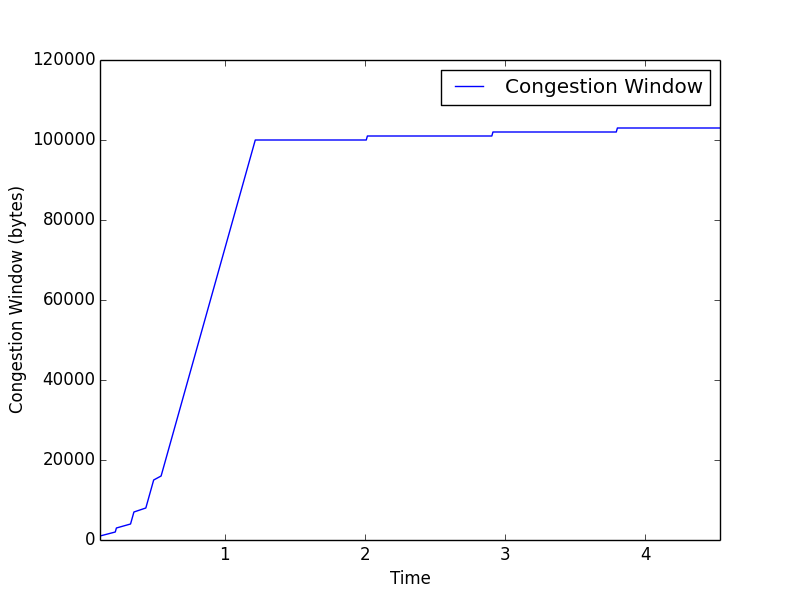
\includegraphics[width=14cm]{graphs/cwnd0loss.png}
\newpage
\item One packet loss: The file was transferred with packet number 14000 dropped. The threshold was reset quite low after the loss, so the majority of cwnd increase is additive. \\
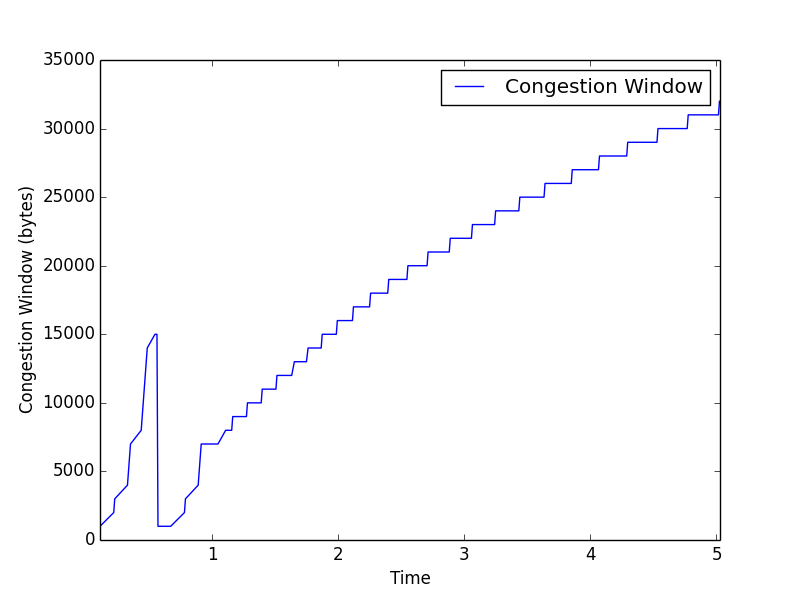
\includegraphics[width=14cm]{graphs/cwnd1loss.png} \\
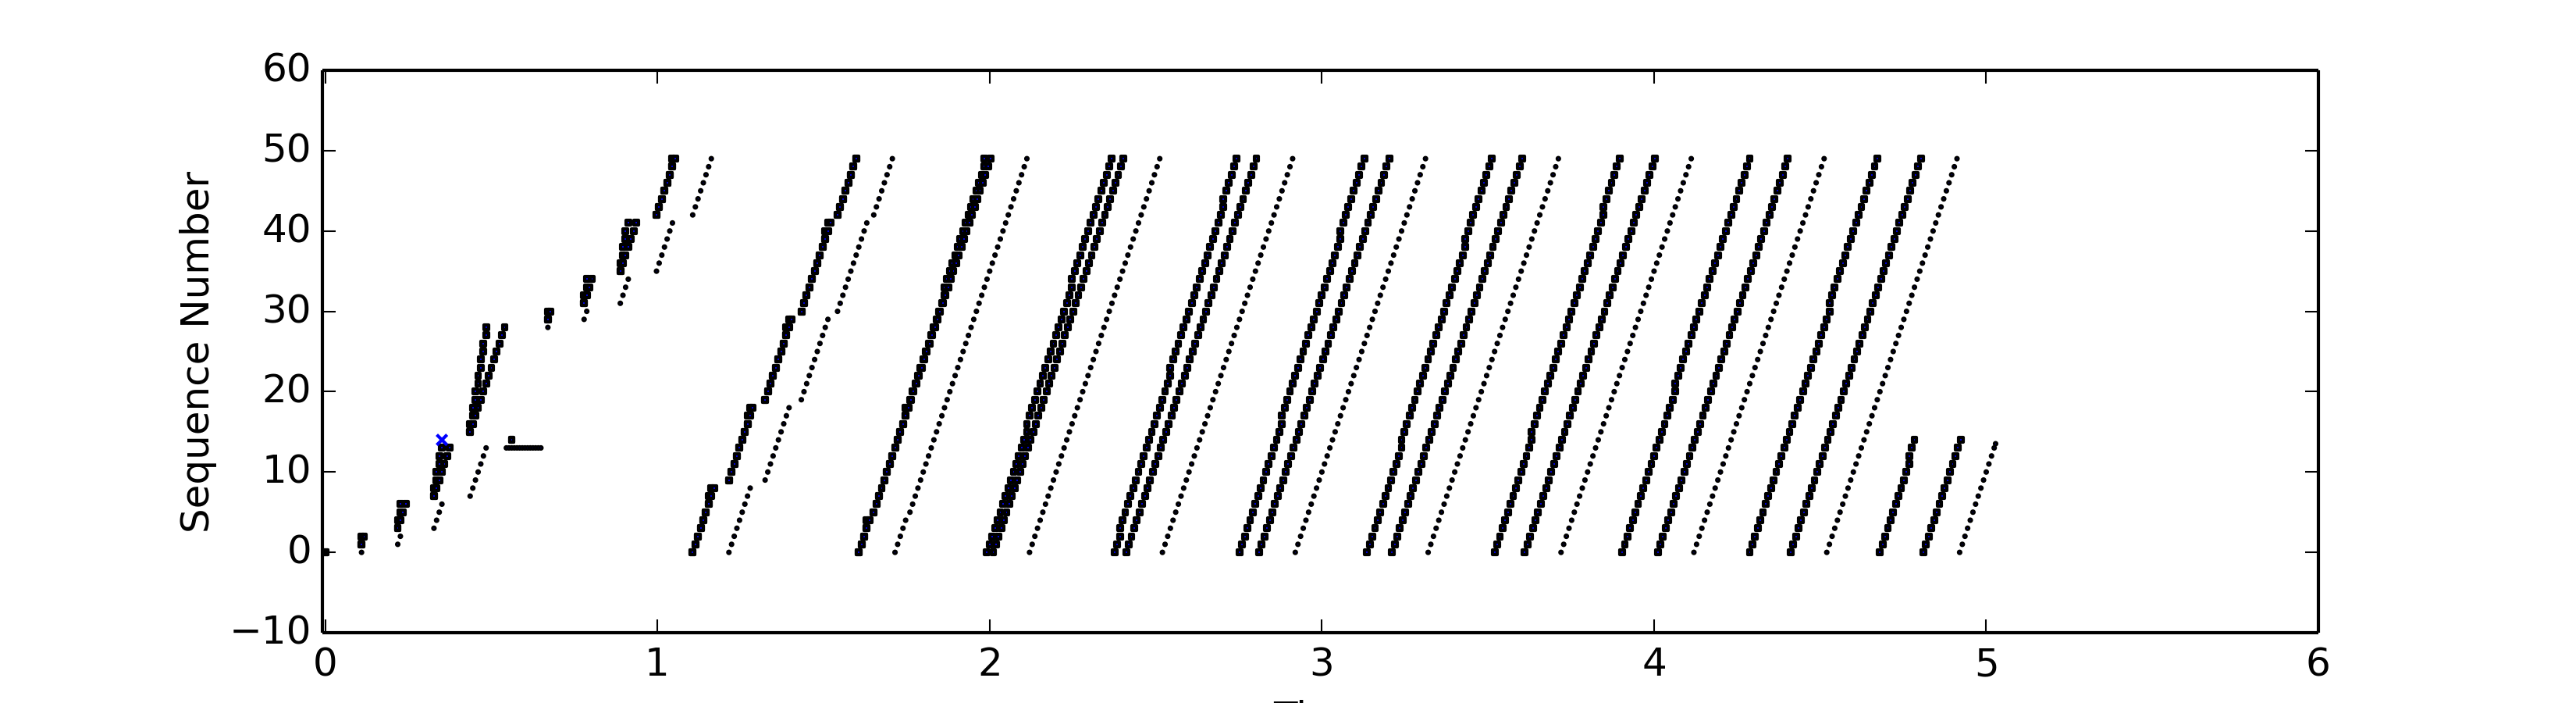
\includegraphics[width=16cm]{graphs/sequence1loss.png}
\newpage
\item Two packet loss: The file was transferred with packets 14000 and 28000 dropped. There is not a noticeable change in the cwnd graph from the test of a single lost packet, because the second packet was dropped within the first packet's congestion window. Retransmit began at 14000, and automatically retransmitted 28000, resulting in only one noticeable loss. \\
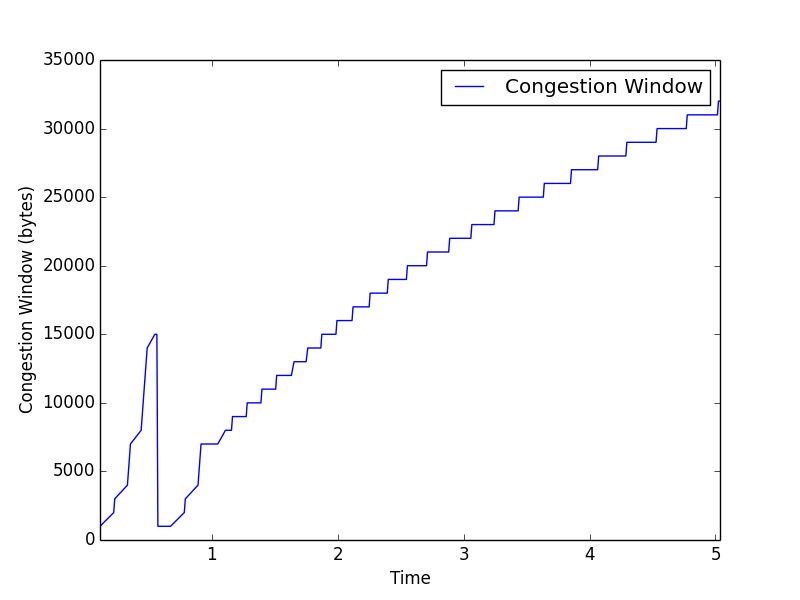
\includegraphics[width=14cm]{graphs/cwnd2loss.png} \\
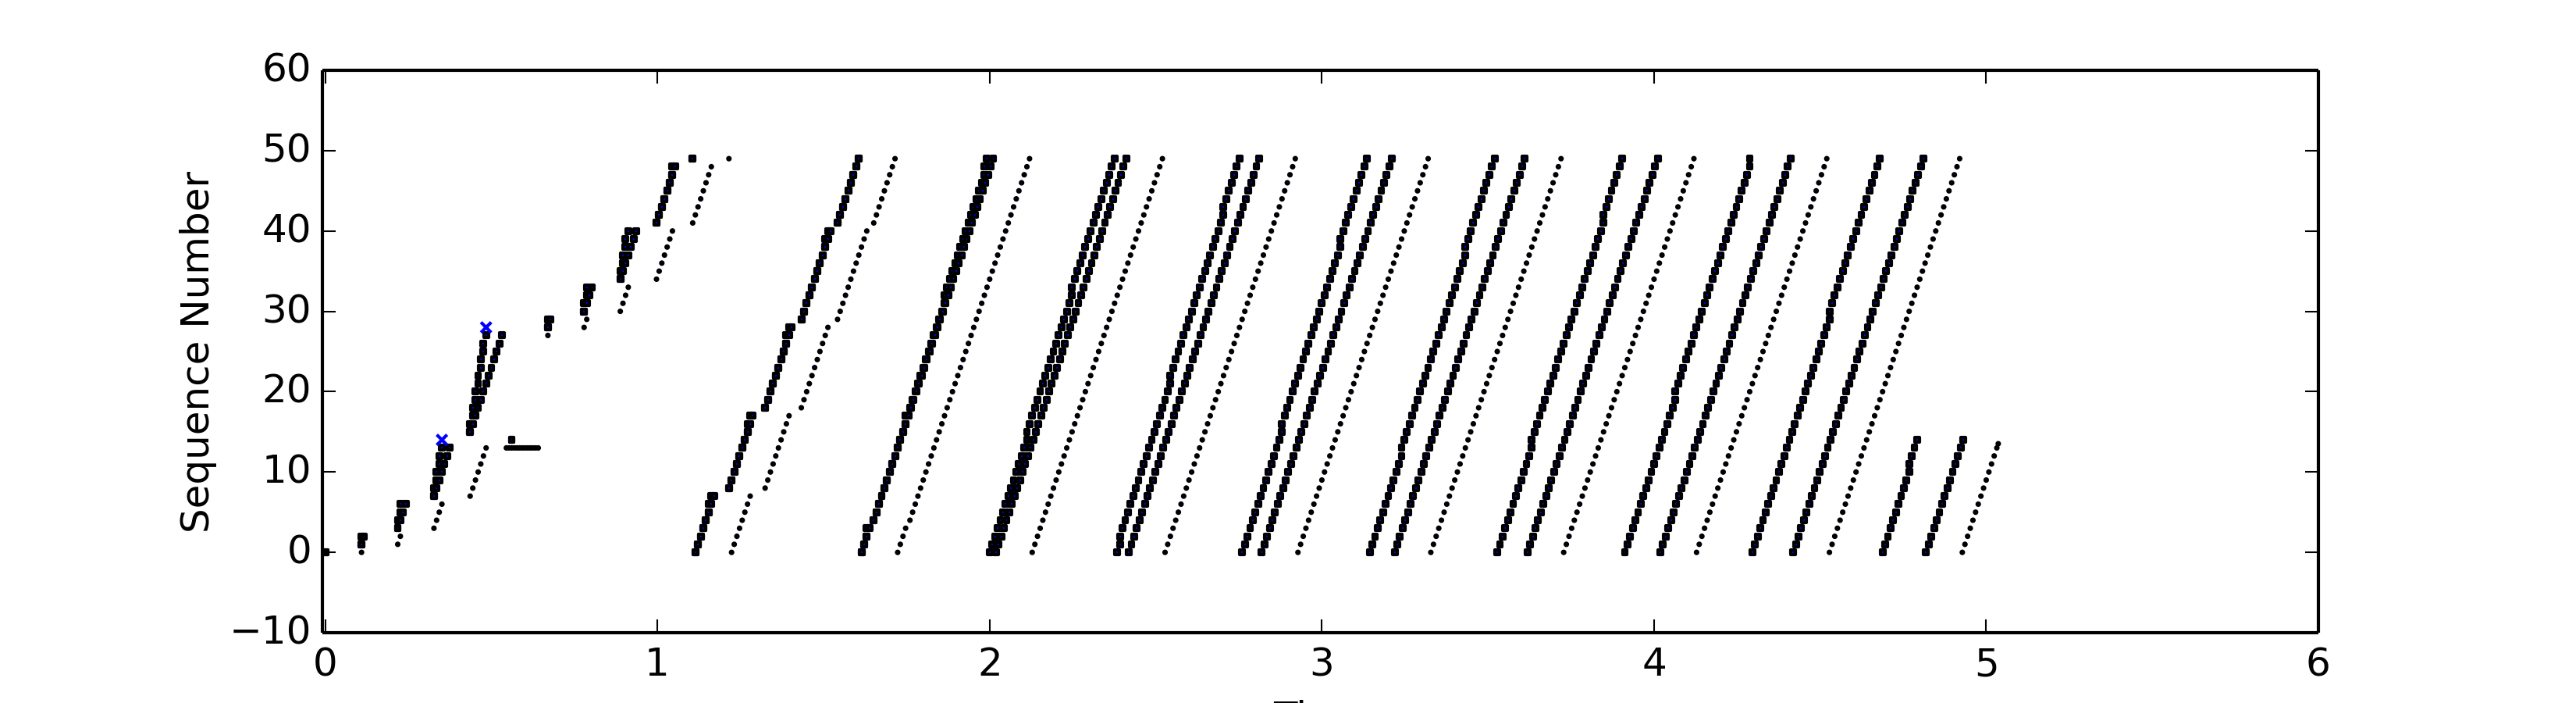
\includegraphics[width=16cm]{graphs/sequence2loss.png}
\newpage
\item Three packet loss: The file was transferred with packets 14000, 26000, and 28000 dropped. Like the test of two lost packets, this situation does not greatly differ from a single packet loss. Again, the subsequent losses are within the window of the first loss, so there is only one loss worth of delay. \\
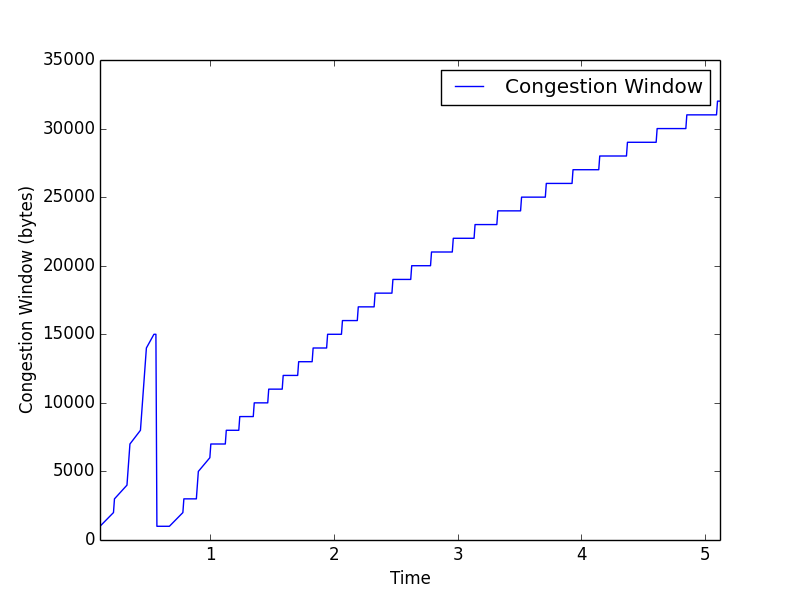
\includegraphics[width=14cm]{graphs/cwnd3loss.png} \\
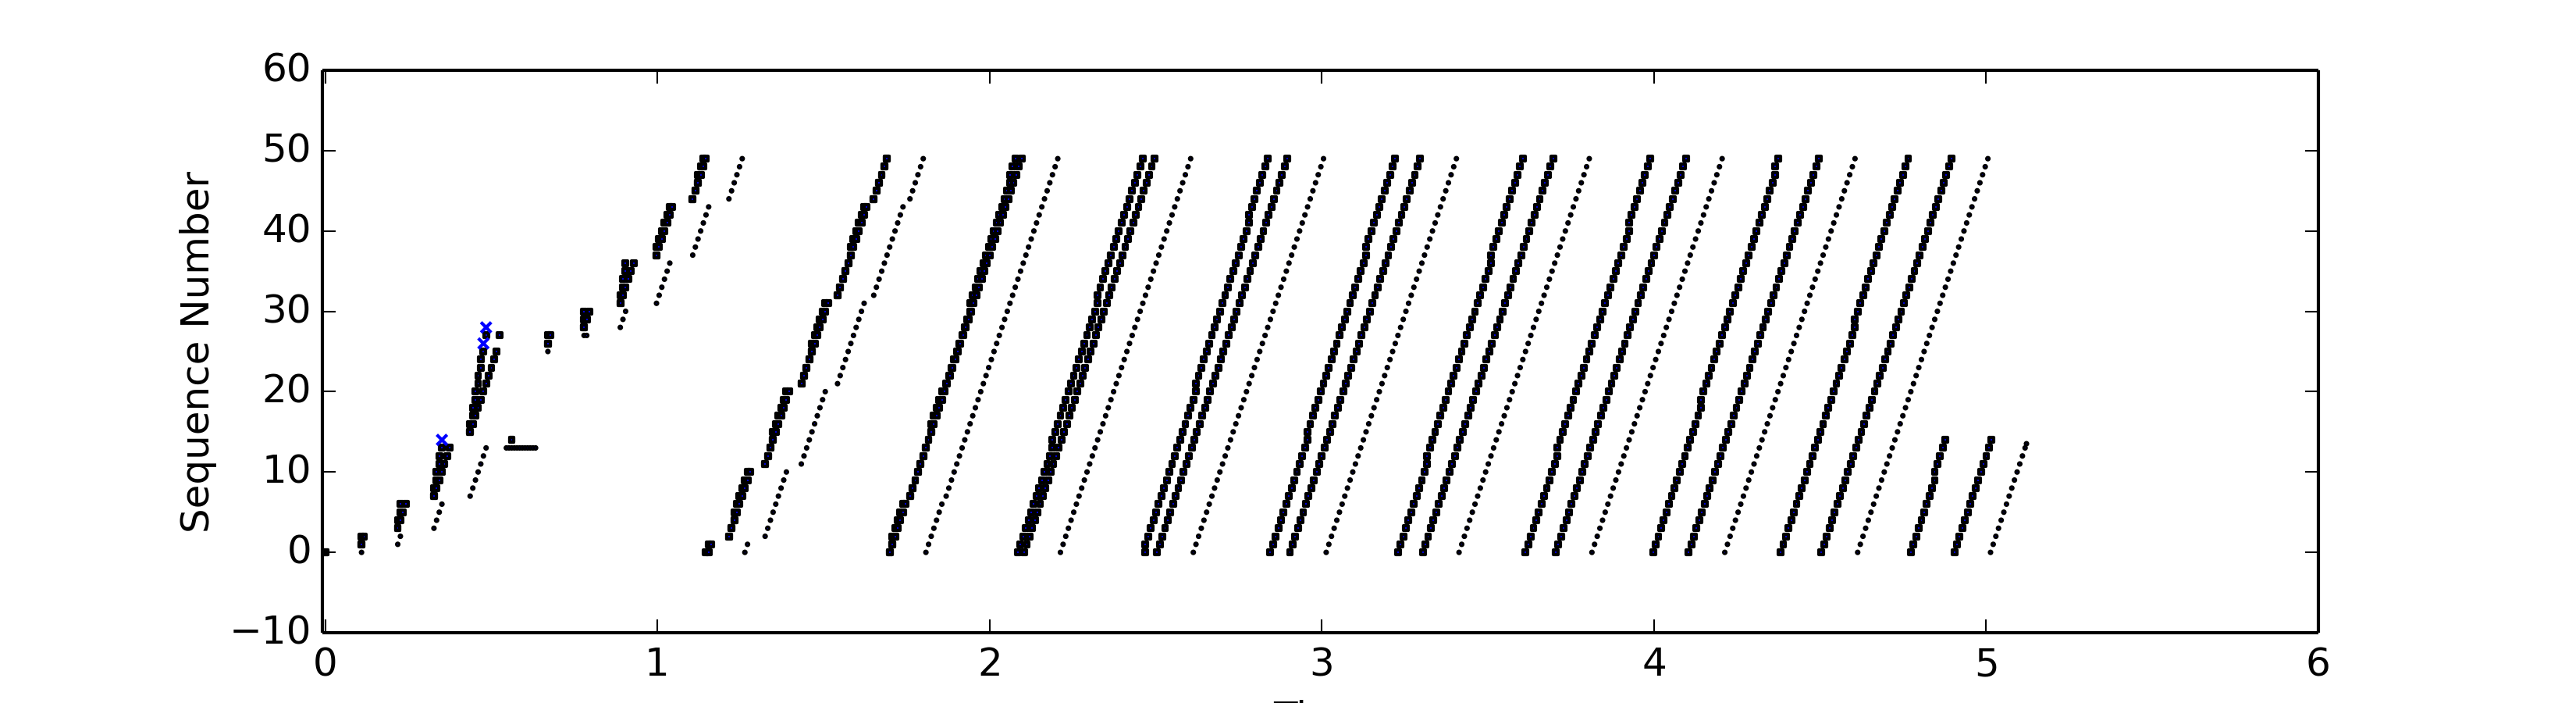
\includegraphics[width=16cm]{graphs/sequence3loss.png}

\end{enumerate}
\newpage
\section{Bonus Test}

I decided to run another test to demonstrate packet loss in separate congestion windows. Packets 100000 and 300000 were dropped, and without much time spent in additive increase, a nice logarithmic decrease can be seen in the cwnd graph. It was fun to experiment with different packet losses in creating this test. \\

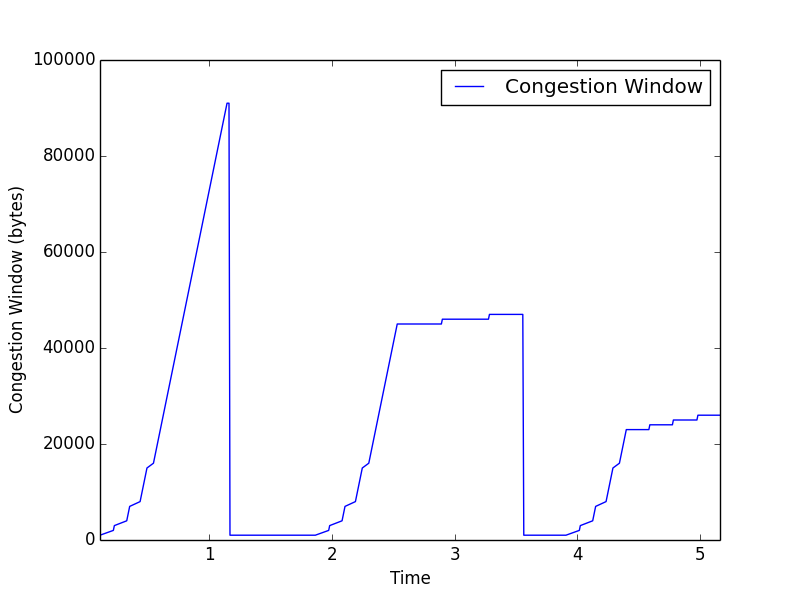
\includegraphics[width=14cm]{graphs/cwnd.png} \\
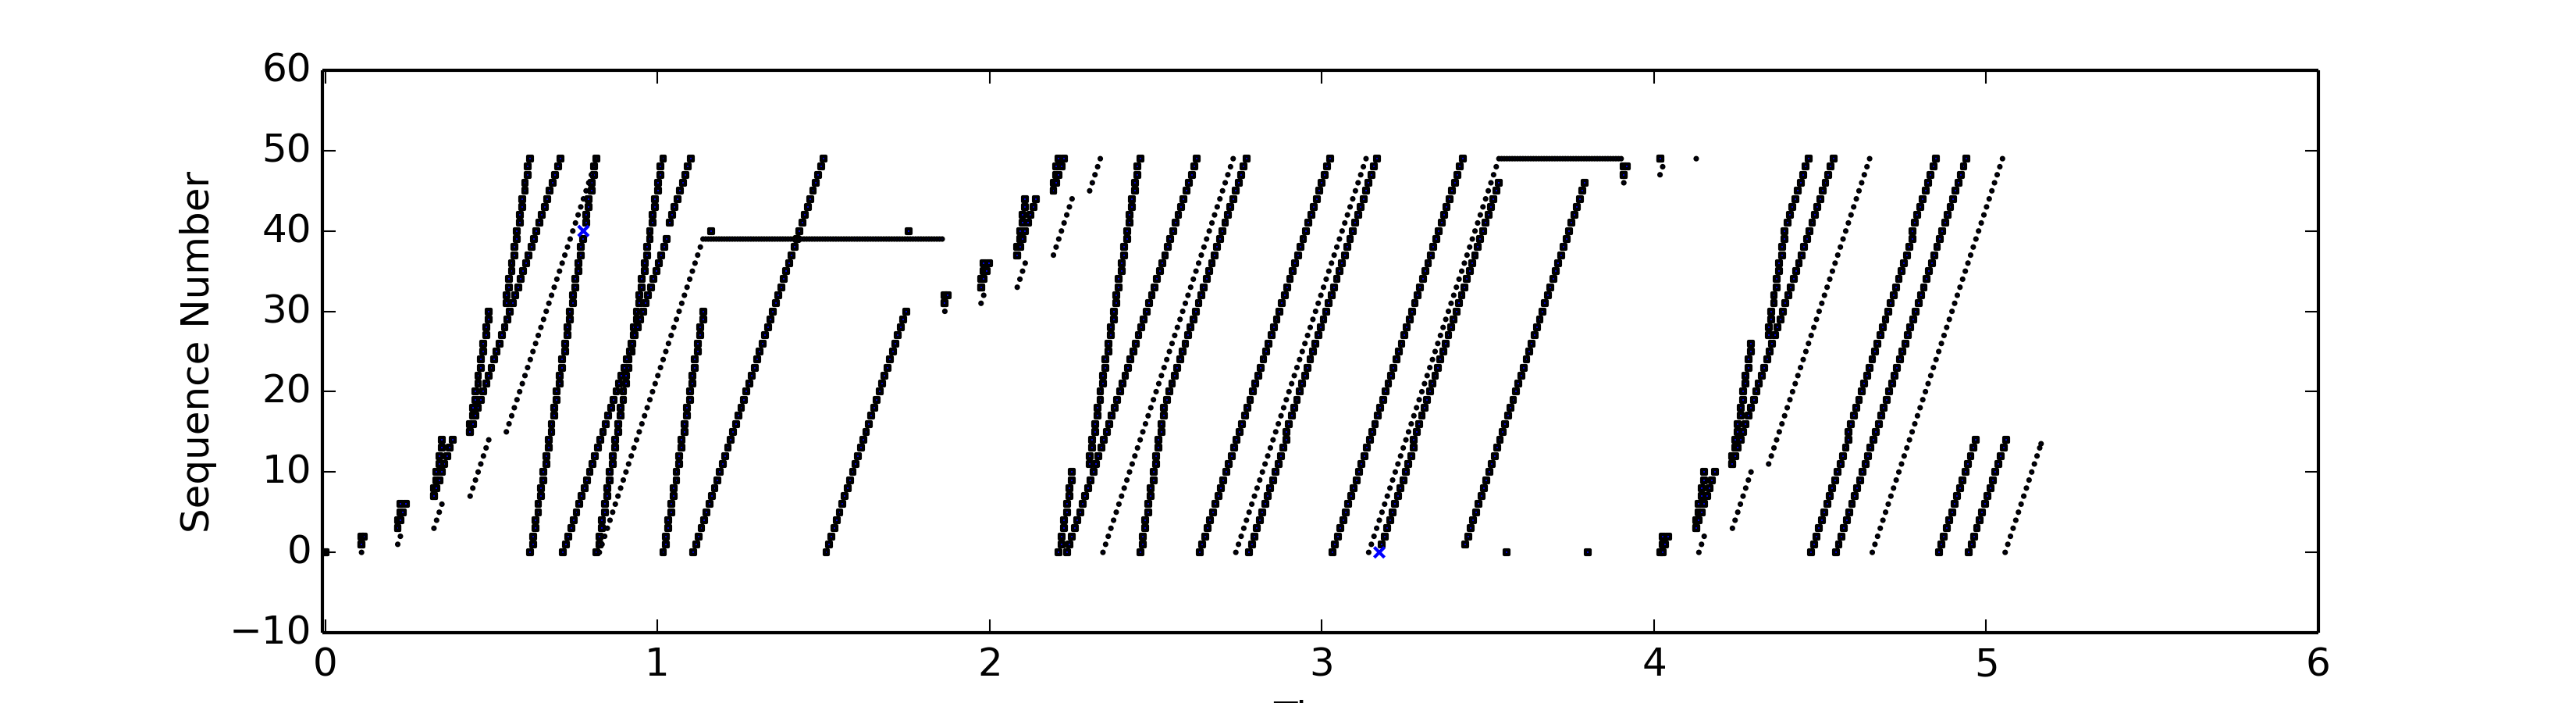
\includegraphics[width=16cm]{graphs/sequence.png}

\end{document}
